\begin{figure}
\begin{center}
\begin{minipage}[t]{\linewidth}

% \hspace*{\fill}%
\begin{minipage}[t]{\linewidth}
\centering
\vspace{0pt} % for alignment
\begin{minipage}{\textwidth}
{\hfil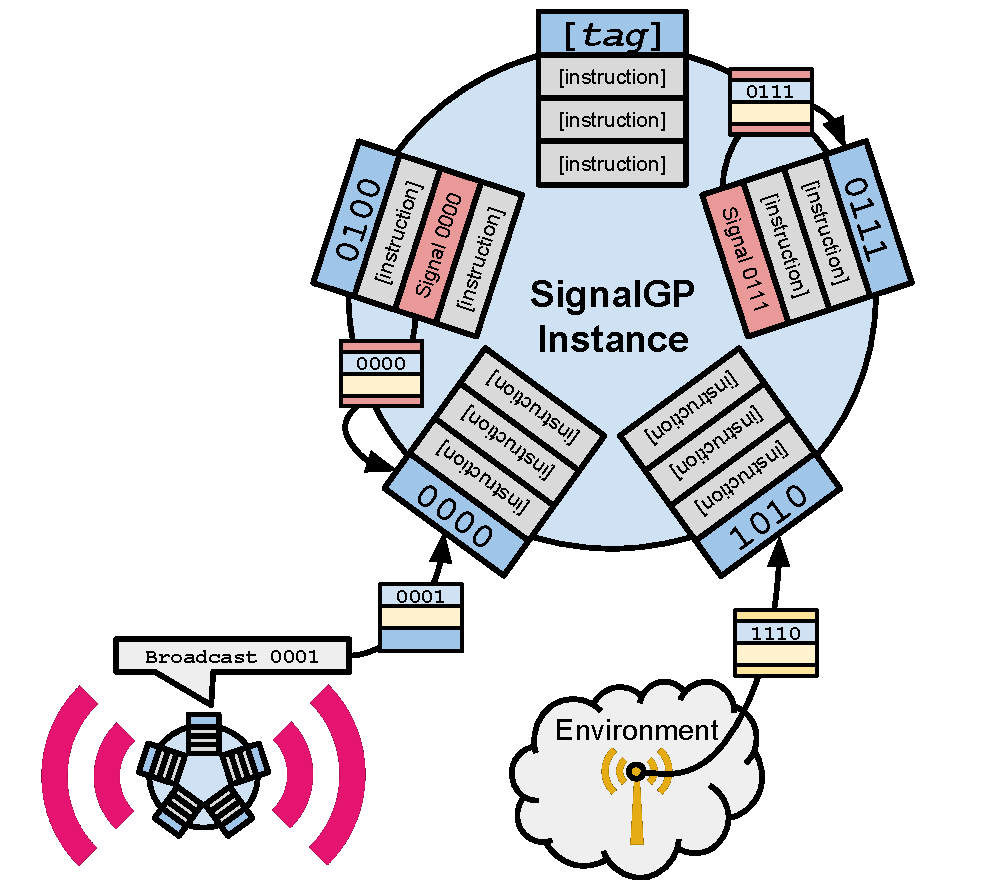
\includegraphics[width=0.5\linewidth]{img/signalgp-cartoon}\hfil}\\
{\textbf{(A)}
Overview of a single SignalGP instance.
SignalGP program modules contain ordered sets of instructions that activate and execute independently in response to tagged signals.
Above, these modules are shown as rectangular lists with bitstring tags protruding from the SignalGP instance.
These signals can originate from any of three sources:
\begin{enumerate}
  \item internally from execution of ``Signal'' instructions within a program's modules,
  \item from the outside environment,
  \item or from other agents executing ``Message'' instructions.
\end{enumerate}
}
% \label{fig:signalgp-cartoon}
\end{minipage}
\end{minipage}%
% \hspace*{\fill}

% \hspace*{\fill}%
% \begin{minipage}[t]{\linewidth}
% \centering
% \vspace{0pt} % for alignment
% \begin{minipage}{\textwidth}
{\hfil
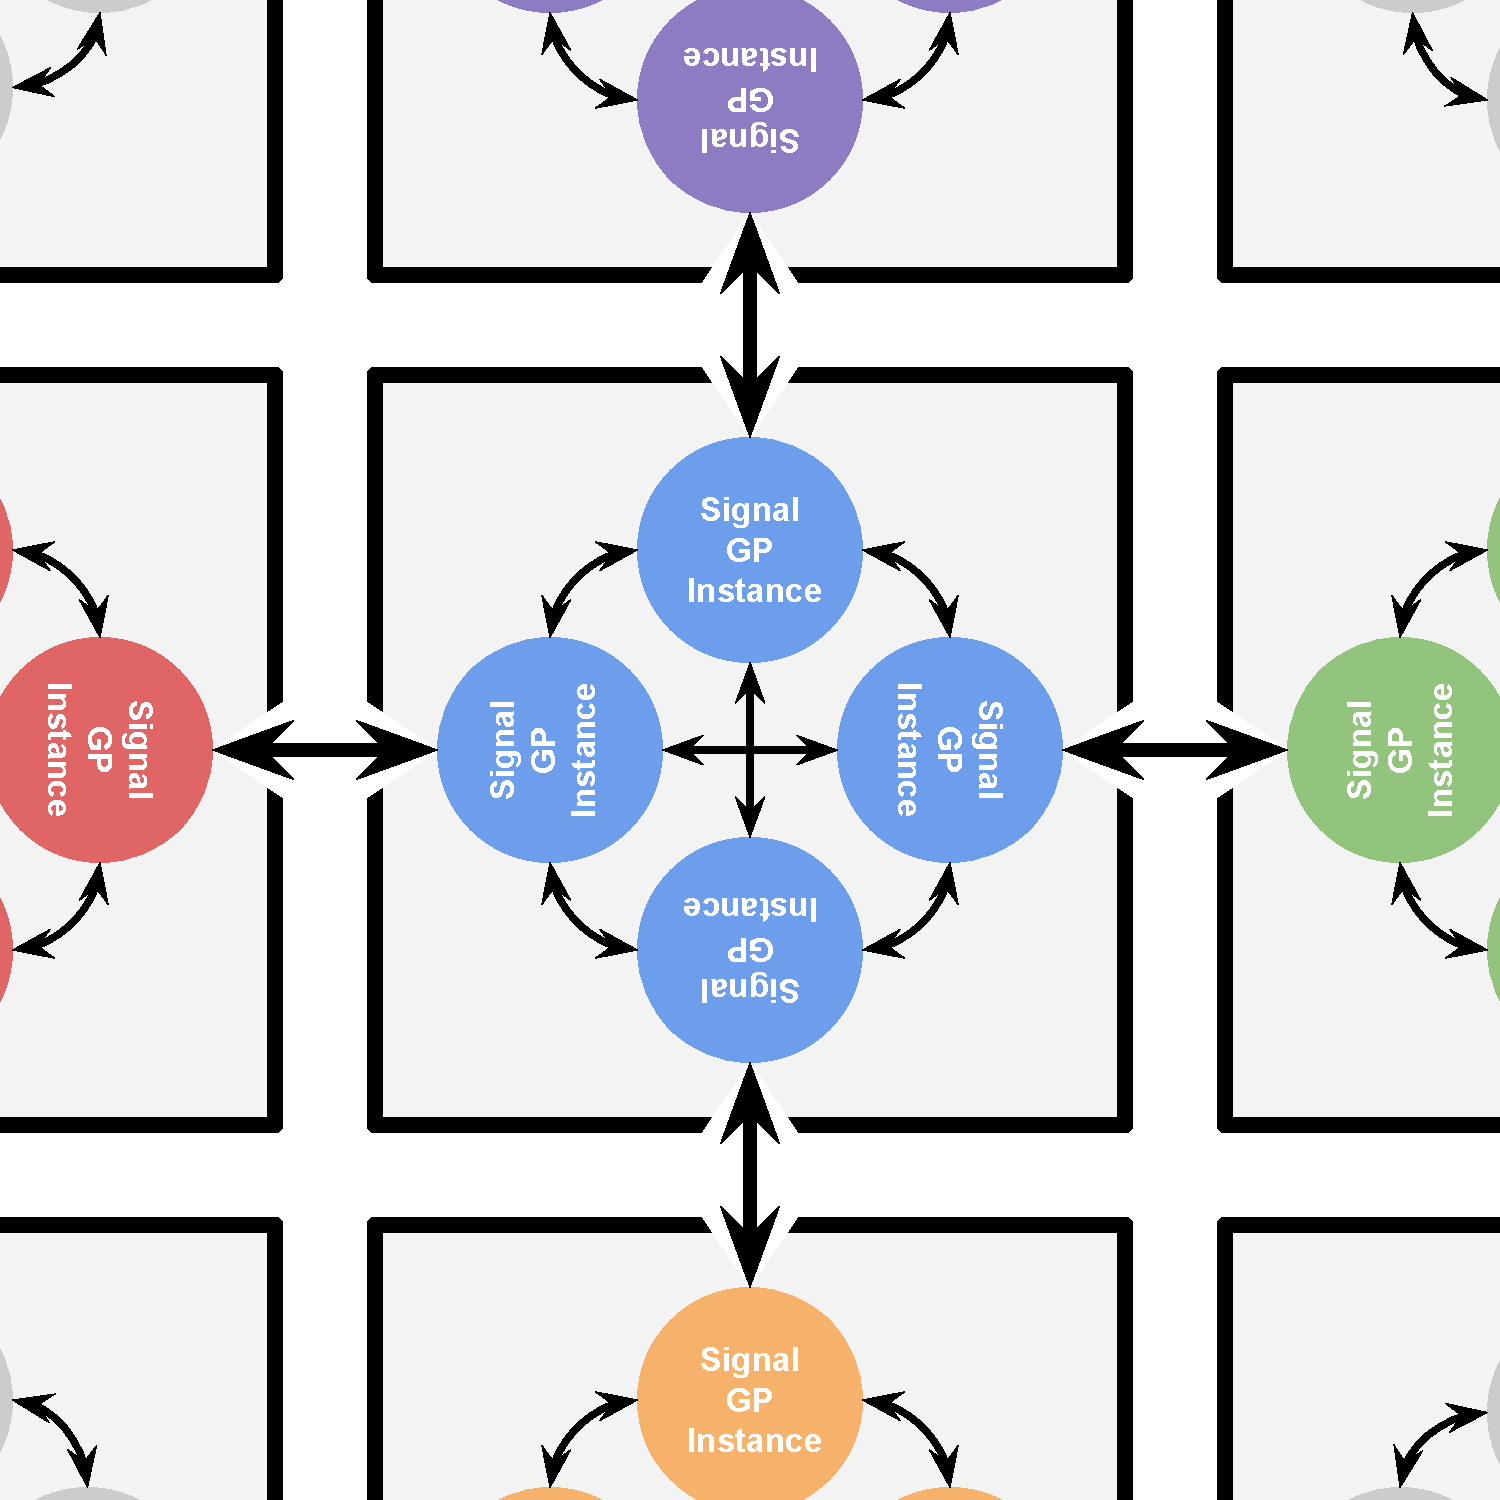
\includegraphics[width=0.45\linewidth]{img/dishtinygp-cartoon}\hfil%
}\\
{\textbf{(B)}
How individual SignalGP instances are organized into DISHTINY cells.
Above, DISHTINY cells are depicted as gray squares.
Each DISHTINY cell is controlled by independent execution of the cell's genetic program on four distinct SignalGP instances, depicted as colored circles.
Each of four independent instances manages cell behavior with respect to a single cardinal direction: sensing environmental state, receiving intercellular messages, and determining cell actions.
Above, the special role of each instance is depicted as a reciporical arrow to the neighboring instance in the neighboring cell.
(All four instances sense non-directional environmental cues and non-directional actions may be taken by any instance.)
These four instances can communicate with one another via a cell communicate via intracellular messaging, indicated above by smaller reciprocal arrows among instances within a cell.
}
% \label{fig:dishtinygp-cartoon}
% \end{minipage}
% \end{minipage}%
% \hspace*{\fill}
\end{minipage}

\caption{
Schematic illustrations of how an individual SignalGP instance functions and how SignalGP instances control DISHTINY cells.
Execution of cells' genetic programs on SignalGP instances controls cell behavior in our model.
Subfigure \textbf{(A)} provided courtesy Alexander Lalejini.
}
\label{fig:signalgp-dishtinygp}
\end{center}
\end{figure}
